\documentclass[amsmath,amssymb,notitlepage,12pt]{revtex4-1}
\usepackage{graphicx}
\usepackage{bm}% bold math
\usepackage{multirow}
\usepackage{booktabs}
\usepackage{verbatim}
\usepackage{hyperref}
\hypersetup{pdftex,colorlinks=true,allcolors=blue}
\usepackage{hypcap}
%\usepackage[small,compact]{titlesec}
%\usepackage{showkeys}
%\addtolength{\textheight}{0.3cm}
%\addtolength{\topmargin}{-0.15cm}
%\addtolength{\textwidth}{0.4cm}
%\addtolength{\hoffset}{-0.2cm}
\begin{document}
%\hspace*{11.5cm}\texttt{HPS-NOTE 2016-XXX}

\title{Cluster-Track Matching}
\author{N. Baltzell, R. Paramezuryan}
%\affiliation{Jefferson Lab}
\date{\today}
\begin{abstract}
    For the HPS 2015 Engineering Run a simple geometrical matching algorithm was implemented based on cluster and extrapolated track $x/y$ positions at the front face of the calorimeter.  Matching quality is parameterized in terms of momentum separately for electrons and positrons, detector halves, and seed and GBL tracks.  The resulting normalized matching quality factor is saved in the reconstruction output with each \texttt{ReconParticle} for use in offline analyses.
\end{abstract}
\maketitle

\section{Residual Measurements}
\subsection{Event Selection}
Events are selected that contain exactly one positively and one negatively charged track with good track quality, one in each half of the detector, and two clusters, again with one in each half of the detector.  The clusters' reconstructed positions are required to be at least $\frac{3}{4}$ of a crystal from the edge of the calorimeter to avoid the region where cluster reconstruction degrades rapidly.  The track trajectory is extrapolated to the front face of the calorimeter using swimming in \texttt{hps-java} and the full 3-D field map.

\subsection{Parameterization}
The residual between the cluster and exptrapolated track positions is modeled with a gaussian on a linear background and fit in momentum bins between 100 and 750 MeV.  The momentum dependence of the mean $\mu$ and width $\sigma$ of the gaussian are then fit with a 5$^{th}$ order polynomial.  This procedure is performed independently for the $x$ and $y$ coordinates, two detector halves, two particle charges, and seed and GBL tracks.

\subsubsection{Features}
\begin{itemize}
    \item In all cases the resolution worsens at low energy due to multiple scattering and degradation of the calorimeter position resolution as the number of crystals in the cluster decreases.
    \item The GBL tracks result in a noticeably better resolution than seed tracks, and resolution is also dependent on track $\chi^2$.
    \item When using a simple 1-D field for track extrapolation to the calorimeter, electrons and positrons showed different offsets at high momentum.  However, in the final parameterization described here with full 3-D field extrapolation, $e^-e^+$  converge to the same offset.  
    \item The 3-D field extrapolation also results in less momentum-dependence of the residuals than for a 1-D field.
\end{itemize}

\section{Matching Algorithm}
The parameterizations of the position residuals in the previous section are implemented in the \texttt{hps-java} reconstruction software and used to determine track-cluster matching quality with an $n_\sigma$ parameter,
\begin{equation}
    n_\sigma^2 = \left[\frac{\mu_x(p)-\delta_x}{\sigma_x(p)}\right]^2 + \left[\frac{\mu_y(p)-\delta_y}{\sigma_y(p)}\right]^2,
    \label{eq:nsigma}
\end{equation}
where $\delta$ is the difference between a particular track's and cluster's measured positions $(x,y)$, and the parameterized residual $(\mu,\sigma)$ is evaluated at that track's momentum $p$.  This calculation is done in \texttt{org.hps.recon.utils.TrackClusterMatcher}.

For each reconstructed track, all clusters in that same detector half are considered and used to calculate their $n_\sigma$ for that track.  The cluster with the smallest $n_\sigma$ less than 30 is then associated with that track.  After all such track and cluster combinations are exhausted, if a track still has no associated cluster then it is assumed to be a photon.  
The particle charge (-1,0,1) determined by track association is then used to perform position and energy corrections for each cluster.  This matching logic is implemented in \texttt{org.hps.recon.particle.ReconParticleDriver}.
 
The class \texttt{ReconParticle} contains the matched cluster and tracks, as well as the $n_\sigma$ parameter accessible with the method \texttt{getGoodnessOfPid()}. 

{\em For analyses interested in optimal matching criteria, some additional requirement on $n_\sigma$ should be applied after reconstruction, probably roughly $n_\sigma<5$.}

\subsection{Caveats}
\subsubsection{Photons}
Due to the cut at $n_\sigma=30$, the matching criteria applied for determining particle type for cluster corrections is very loose.  This was chosen in favor of flexible $e^+e^-$ analyses and not well suited for analyses where optimal photon energy and position reconstruction are needed.
\subsubsection{Cluster Corrections}
Matching quality is evaluated before cluster position corrections are applied.  Since the residual parameterizations were also extracted before cluster position corrections and are charge-dependent, the final matching determination is not significantly affected.  However, applying the corrections based on the corresponding track's charge before evaulating matching quality might narrow the residuals and resulting $n_\sigma$ distribution and allow to reduce the background under the $n_\sigma$ peak.
\subsubsection{Edge Effects}
Near the beam gap the cluster $y$-position resolution degrades rapidly and becomes just the crystal position when the particle enters much less than a half crystal from the edge.  This is not accounted for in this work.  The effect can be seen in Figure~\ref{fig:nsigmay} at small-$|y|$, and it is possible to account for this in analyses with a $|y|$-dependent requirement on $n_\sigma$.


\section{Conclusion}
yep.

\begin{figure}[htbp]\centering
    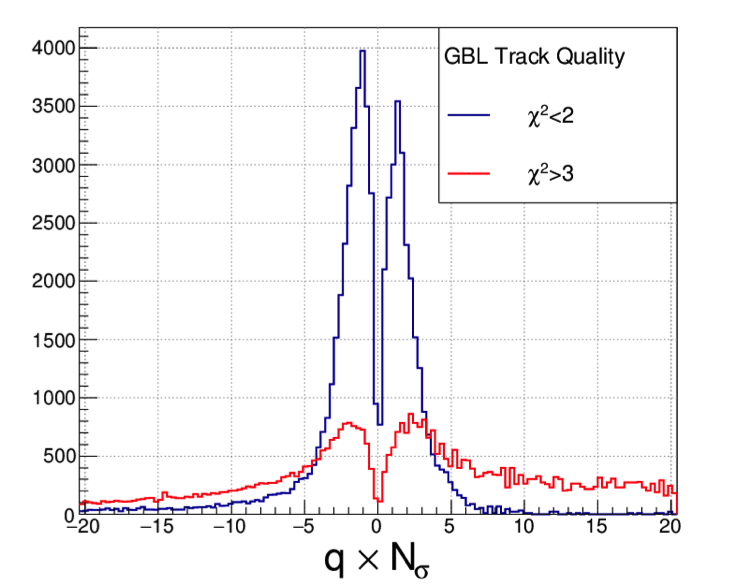
\includegraphics[width=0.7\textwidth]{pics/qnsx2}
    \caption{$n_\sigma$ distrubtion for electrons and positrons for different ranges of track $\chi^2$.  Positrons are scaled up by a factor of 10 for visualization, and $n_\sigma$ is multiplied by particle charge ($\pm1$) to separate positrons and electorons.\label{fig:nsigma}}
\end{figure}

\begin{figure}[htbp]\centering
    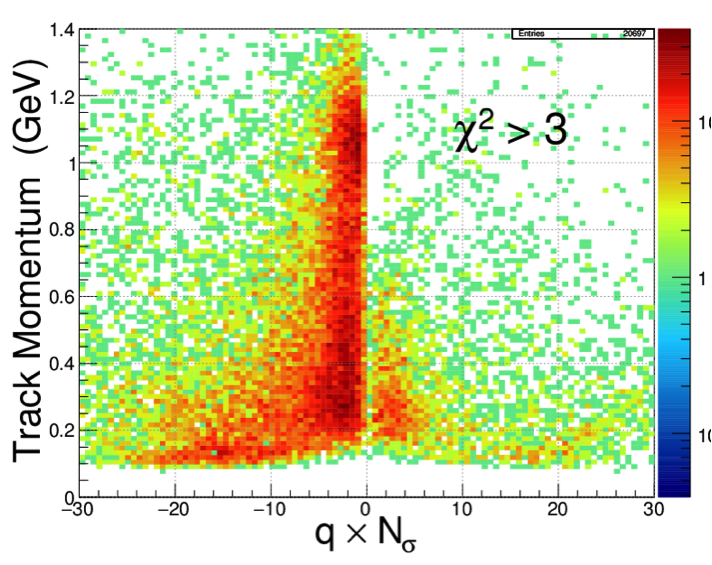
\includegraphics[width=0.49\textwidth]{pics/qnspx2lo}
    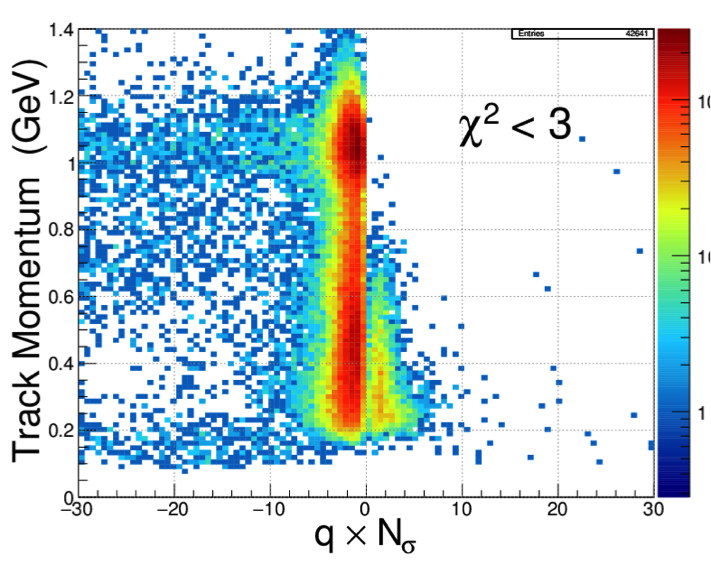
\includegraphics[width=0.49\textwidth]{pics/qnspx2hi}
    \caption{$n_\sigma$ versus momentum for low (left) and high (right) values of track $\chi^2$.  $n_\sigma$ is multiplied by particle charge ($\pm1$) to separate positrons and electrons.\label{fig:nsigmap}}
\end{figure}

\begin{figure}[htbp]\centering
    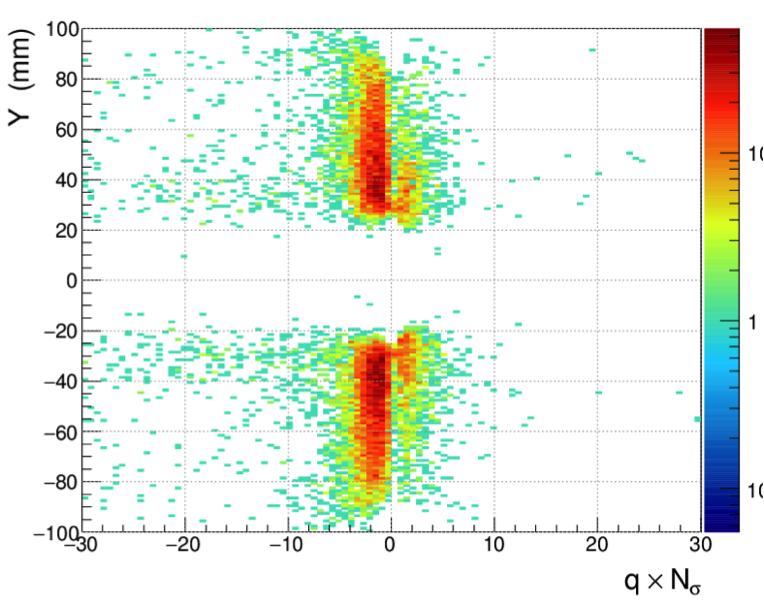
\includegraphics[width=0.49\textwidth]{pics/qnsyplo}
    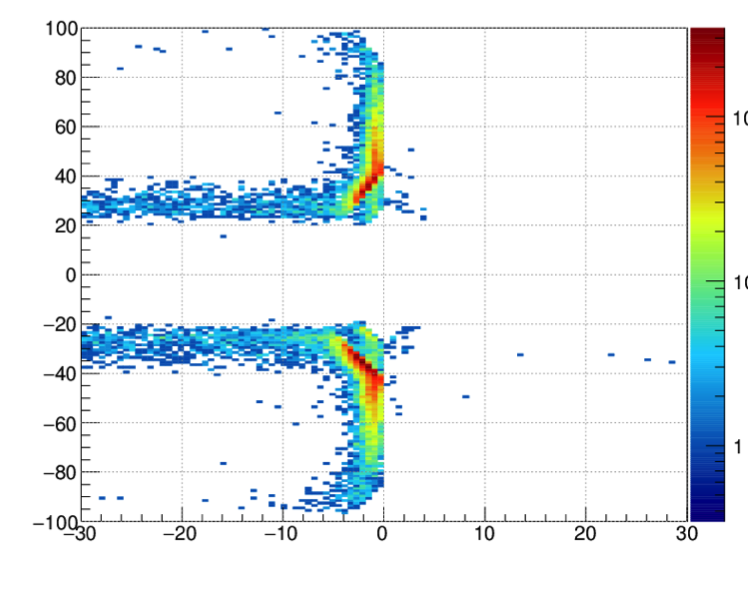
\includegraphics[width=0.49\textwidth]{pics/qnsyphi}
    \caption{$n_\sigma$ versus track $y$-position at the calorimeter for low (left) and high (right) momentum.  $n_\sigma$ is multiplied by particle charge ($\pm1$) to separate positrons and electrons.\label{fig:nsigmay}}
\end{figure}


%\appendix
%\section{Parameterizations}
%The means and sigmas of the cluster-track distributions are parameterized as $5^{th}$ order polynomials,
%$(p_0*(p_1+p*(p_2+p*(p_3+p*(p_4+p(p_5))))))$, with the parameters defined in the table.
%
%\begin{table}[htbp]\centering
%    \begin{tabular}{rccccccc} \hline
%        && $p_0$ & $p_1$ & $p_2$ & $p_3$ & $p_4$ & $p_5$ \\ \hline
%        \multirow{6}{*}{Top}&\multirow{3}{*}{$e^+$}       & $p_0$ & $p_1$ & $p_2$ & $p_3$ & $p_4$ & $p_5$ \\
%               && $p_0$ & $p_1$ & $p_2$ & $p_3$ & $p_4$ & $p_5$ \\
%               && $p_0$ & $p_1$ & $p_2$ & $p_3$ & $p_4$ & $p_5$ \\ \cmidrule[1pt]{2-8}
%               &\multirow{3}{*}{$e^-$}& $p_0$ & $p_1$ & $p_2$ & $p_3$ & $p_4$ & $p_5$ \\
%               && $p_0$ & $p_1$ & $p_2$ & $p_3$ & $p_4$ & $p_5$ \\
%               && $p_0$ & $p_1$ & $p_2$ & $p_3$ & $p_4$ & $p_5$ \\ \cmidrule[1.5pt]{1-8}
%        \multirow{6}{*}{Bottom}&\multirow{3}{*}{$e^-$}       & $p_0$ & $p_1$ & $p_2$ & $p_3$ & $p_4$ & $p_5$ \\
%               && $p_0$ & $p_1$ & $p_2$ & $p_3$ & $p_4$ & $p_5$ \\
%               && $p_0$ & $p_1$ & $p_2$ & $p_3$ & $p_4$ & $p_5$ \\ \cmidrule[1pt]{2-8}
%               &\multirow{3}{*}{$e^-$}& $p_0$ & $p_1$ & $p_2$ & $p_3$ & $p_4$ & $p_5$ \\
%               && $p_0$ & $p_1$ & $p_2$ & $p_3$ & $p_4$ & $p_5$ \\
%               && $p_0$ & $p_1$ & $p_2$ & $p_3$ & $p_4$ & $p_5$ \\ \cmidrule[1.5pt]{1-8}
%    \end{tabular}
%    \caption{\label{}}
%\end{table}
%
%private static final double dxMeanTopPosiGBL[] = { 6.67414,-9.57296, 5.70647, 27.4523,-28.1103,-9.11424 };
%    private static final double dxSigmTopPosiGBL[] = { 52.6437,-478.805, 1896.73,-3761.48, 3676.77,-1408.31 };
%    private static final double dxMeanBotPosiGBL[] = { 4.13802, 15.8887,-74.2844,-9.78944, 308.541,-287.668 };
%    private static final double dxSigmBotPosiGBL[] = { 37.6513,-294.851, 1002.15,-1639.08, 1228.02,-308.754 };
%
%    private static final double dxMeanTopElecGBL[] = {-1.6473,  5.58701, 25.3977,-17.1523,-121.025, 145.969 };
%    private static final double dxSigmTopElecGBL[] = { 48.7018,-423.599, 1592.66,-2959.99, 2668.97,-919.876 };
%    private static final double dxMeanBotElecGBL[] = {-6.63558, 83.7763,-460.451, 1275.63,-1702.83, 873.913 };
%    private static final double dxSigmBotElecGBL[] = { 47.0029,-411.784, 1586.52,-3083.37, 2985.58,-1145.53 };
%
%    private static final double dyMeanTopPosiGBL[] = { 0.31245, 5.57585,-6.50267,-8.21688, 39.8607,-43.9661 };
%    private static final double dySigmTopPosiGBL[] = { 33.0213,-275.174, 1168.77,-2642.34, 3045.52,-1406.21 };
%    private static final double dyMeanBotPosiGBL[] = {-7.032,   74.9738,-383.972, 977.849,-1250.28, 637.75  };
%    private static final double dySigmBotPosiGBL[] = { 19.019, -83.9253, 133.813, 119.883,-546.951, 405.207 };
%
%    private static final double dyMeanTopElecGBL[] = { 2.48498,-20.4101, 62.9689, 25.6386,-259.957, 207.145 };
%    private static final double dySigmTopElecGBL[] = { 8.65583, 120.676,-1166.43, 3811.72,-5383.19, 2787.42 };
%    private static final double dyMeanBotElecGBL[] = {-10.5228, 112.329,-489.761, 953.037,-829.96,  260.772 };
%    private static final double dySigmBotElecGBL[] = { 23.4856,-108.19,  158.7,   189.261,-682.034, 459.15  };
%
%    private static final double dxMeanTopPosiSeed[] ={ 11.6245,-28.5061, 13.0332, 59.9465,-21.1014,-63.6126 };
%    private static final double dxSigmTopPosiSeed[] ={ 61.5911,-540.596, 2077.22,-3973.22, 3704.45,-1332.07 };
%    private static final double dxMeanBotPosiSeed[] ={ 4.53394, 11.3773,-63.7127,-2.81629, 273.868,-264.709 };
%    private static final double dxSigmBotPosiSeed[] ={ 48.3163,-409.249, 1590.36,-3212.85, 3326.04,-1402.3  };
%
%    private static final double dxMeanTopElecSeed[] ={ 2.14163,-20.8713, 76.3054,  34.894,-340.272,  295.24 };
%    private static final double dxSigmTopElecSeed[] ={ 48.585, -385.166, 1320.26,-2157.45, 1581.06,-366.012 };
%    private static final double dxMeanBotElecSeed[] ={-3.44302, 12.4687, 4.09878,-30.0057,-13.3151, 40.2707 };
%    private static final double dxSigmBotElecSeed[] ={ 48.4089,-385.494, 1341.37,-2271.52, 1814.02,-526.555 };
%
%    private static final double dyMeanTopPosiSeed[] ={-0.527741,10.4944, -18.242,-12.9155, 81.0116,-73.9773 };
%    private static final double dySigmTopPosiSeed[] ={ 37.3097, -357.55, 1607.03,-3709.55, 4282.36,-1957.91 };
%    private static final double dyMeanBotPosiSeed[] ={ 0.74392,-55.2003,  405.04,-1250.64, 1731.47,-887.262 };
%    private static final double dySigmBotPosiSeed[] ={ 25.5776,-199.731,  754.59,-1408.72, 1240.36,-400.912 };
%
%    private static final double dyMeanTopElecSeed[] ={ 2.85429,-24.0858, 69.0145, 34.1213,-297.752, 239.939 };
%    private static final double dySigmTopElecSeed[] ={ 19.9111,-53.2699,-261.915,  1593.2,-2774.01, 1605.54 };
%    private static final double dyMeanBotElecSeed[] ={-9.22963, 98.1346, -427.91, 840.225,-751.188, 250.792 };
%    private static final double dySigmBotElecSeed[] ={ 21.7909,-85.4757,-56.9423, 977.522,-1902.05, 1137.92 };

\bibliography{clusterTrackMatching}
\end{document}

